% Test tex file!

\documentclass[a4paper,12pt]{article}
\usepackage{times}  % DO NOT CHANGE THIS
\usepackage{helvet} % DO NOT CHANGE THIS
\usepackage{courier}  % DO NOT CHANGE THIS
\usepackage[hyphens]{url}  % DO NOT CHANGE THIS
\usepackage{graphicx} % DO NOT CHANGE THIS
\urlstyle{rm} % DO NOT CHANGE THIS
\def\UrlFont{\rm}  % DO NOT CHANGE THIS
\usepackage{natbib}  % DO NOT CHANGE THIS AND DO NOT ADD ANY OPTIONS TO IT
\usepackage{caption} % DO NOT CHANGE THIS AND DO NOT ADD ANY OPTIONS TO IT
\frenchspacing  % DO NOT CHANGE THIS
\setlength{\pdfpagewidth}{8.5in}  % DO NOT CHANGE THIS
\setlength{\pdfpageheight}{11in}  % DO NOT CHANGE THIS
\usepackage{algorithm} %format of the algorithm 
\usepackage{algorithmic} %format of the algorithm 
\usepackage{multirow} %multirow for format of table 
\usepackage{amsmath} 
\usepackage{xcolor}
\usepackage{amssymb}
\usepackage{amsmath}
\usepackage{CJKutf8}
\usepackage{courier}

\begin{document}

\begin{CJK}{UTF8}{gbsn}
% \begin{CJK}{UTF8}{gkai}

\title{强化学习:作业三}

\author{傅浩敏 MG20370012}

\date{2020年12月9日}

\maketitle

\section{作业内容}
我们需要在gym Atari环境中实现DQN算法及其变体。本实验的实验环境是Atari Game Pong,Agent需要操控球拍与系统互相击球,未接到球则对方计一分,先取得21分者获胜。实验目标是训练DQN及其变体作为Agent获得游戏胜利,并使获胜时的分差尽可能大。在本次实验中,我分别实现和训练了DQN\cite{ref1}、Double DQN\cite{ref2}以及Dueling DQN\cite{ref3},并评估了它们在训练过程中的表现和它们在上述游戏中的性能。同时我也实现了Prioritized Replay Buffer\cite{ref4},但是完整的算法受限于我的硬件性能无法运行,因此我对论文中的算法进行了一定的简化,并且评估了简化后的算法对DQN训练过程的影响。

\section{实现过程}
\subsection{算法描述}
\paragraph{Q-learning\cite{ref5}} 在传统Q-learning算法中,我们使用一张 $Q$ 表来记录环境状态 $s$ 以及该状态对应各个动作 $a$ 的长期回报值 $Q(s,a)$,并使用下式来更新 $Q$ 表:
$$
\begin{cases}
	&a'= \mathop{\arg\max}_{x} Q(s',x)\\
	&Q(s,a)=Q(s,a)+\alpha(r+\gamma Q(s',a')-Q(s,a)) 
\end{cases}
$$
其中 $s'$ 是在状态 $s$ 下执行动作 $a$ 后的新状态,$\alpha$ 和 $\gamma$ 分别为学习率和折扣系数。
\paragraph{DQN} 在DQN中,我们不使用表型数据结构记录 $Q$ 值,而是用一个深度神经网络来计算不同的状态-动作对应的 $Q$ 值。DQN相较于传统的Q-learning算法能更好地处理状态-动作空间较大的场景。在DQN中,我们需要最小化TD error,既使网络输出 $Q(s,a)$ 逼近于长期回报的估计值 $r+\gamma Q(s',\mathop{\arg\max}_{x} Q(s',x))$, 其中 $\gamma$ 为折扣系数。我使用均方误差作为损失函数,因此神经网络优化器需要最小化下式:
$$
\|r+\gamma Q(s',\mathop{\arg\max}_{x} Q(s',x))-Q(s,a)\|_2^2
$$
注意到,我们在改变网络参数的时候也会改变优化目标,因此我们需要复制一份原神经网络作为目标网络,从而使优化目标相对稳定。因此改写损失如下:
$$
\|r+\gamma Q'(s',\mathop{\arg\max}_{x} Q'(s',x))-Q(s,a)\|_2^2
$$
其中 $Q$ 为原网络输出, $Q'$ 为目标网络输出。在经过一段时间的训练后,我们需要将原网络参数复制到目标网络上。
\paragraph{Double DQN} 该变体是对DQN中训练目标的优化。在Q-learning算法中,采用 $\arg\max$ 选择动作会导致对 $Q$ 值的估计有一定程度的偏高\cite{ref2}。Double DQN通过解耦动作选择和 $Q$ 值估计来减少偏差值。即在当前网络上对状态 $s'$ 通过 $\arg\max$ 选择动作 $a'$ ,而在目标网络上计算 $s',\ a'$ 对应的 $Q$ 值。因此可将损失函数改写为:
$$
\|r+\gamma Q'(s',\mathop{\arg\max}_{x} Q(s',x))-Q(s,a)\|_2^2
$$
通过这种方式,可以缓解估计值偏高的问题。
\paragraph{Dueling DQN} 该变体是对DQN中网络结构的优化。在原始DQN中,神经网络模型直接输出了各个动作对应的 $Q$ 值;而在Dueling DQN中,模型的输出会由Value Function和Advantage Function两个子网络的输出相加获得。其中Value Function仅输出对应状态的 $Q$ 值,而Advantage Function则会输出对应状态各个动作对 $Q$ 值的“增益”。通过这种方式可以使网络更加精确地估计 $Q$ 值。
\begin{figure}[h!]
\centering
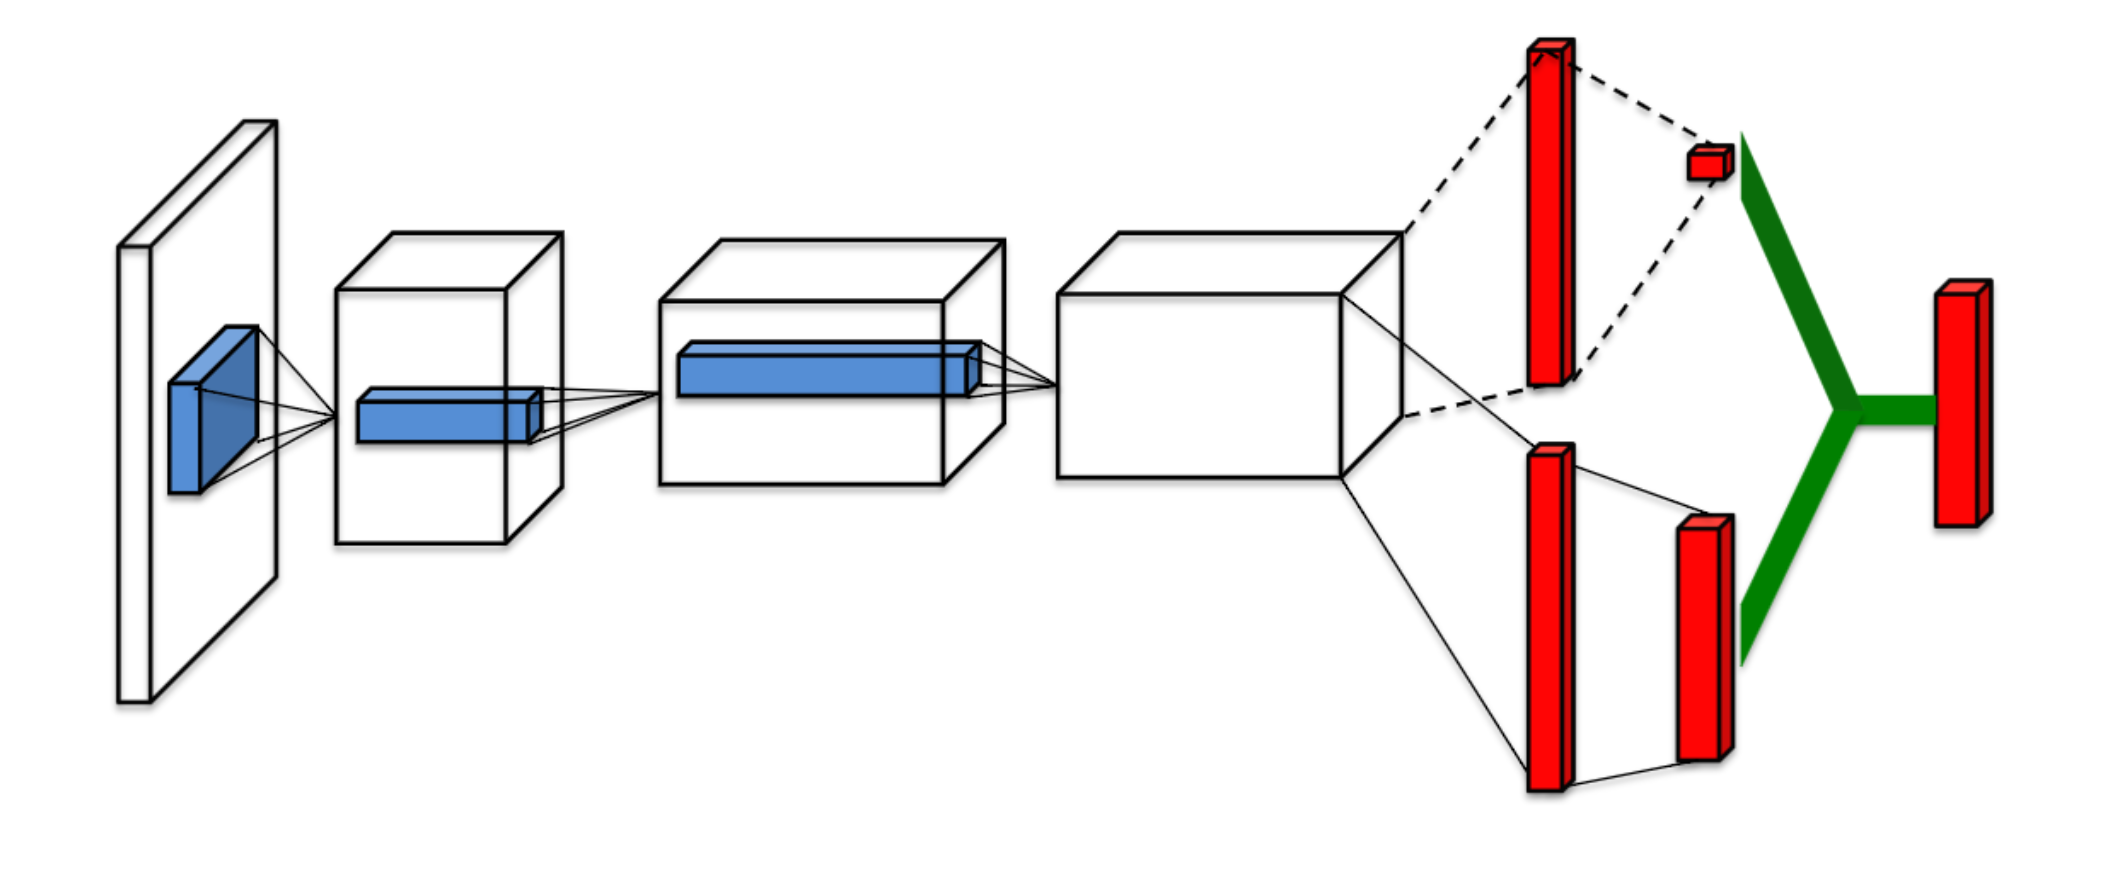
\includegraphics[width=8cm,height=4cm]{./resource/dueling_architecture.png}
\caption{Dueling DQN 网络结构\cite{ref3}}
\end{figure}
\newpage
\subsection{代码实现}
\noindent DQN学习过程伪代码如下:
\begin{algorithm}[!h]
	\caption{DQN learning function}
	\begin{algorithmic}[1]
		\STATE \textbf{Input:} current step $step$,update interval $update$, minibatch $k$, discount rate $\gamma$, sample buffer $buffer$, model $\pi$, target model $\pi'$.
		\STATE Sample state, next state, action, reward and done mask from buffer \\$s0, s1, a, r, done =buffer.sample(k)$
		\STATE Calculate models' outputs $modelOutputs=\pi(s0)$, $targetModelOutputs=\pi'(s1)$
		\STATE Find max value in actions $targetMax$=max($targetModelOutputs$)
		\STATE Calculate target $target$=$r + \gamma*(1-done)*targetMax$
		\STATE Find value of the actions $presentValue=modelOutputs[a]$
		\STATE Calculate MSE loss $loss=\|presentValue-target\|_2^2$
		\STATE Update parameters $\pi.update()$
		\IF{$fr$ mod $update$ == 0}
		\STATE Update target model $\pi'=\pi$
		\ENDIF
	\end{algorithmic}
\end{algorithm}
\\
\noindent Double DQN只在Algorithm 1的基础上优化了动作选择的过程:
\begin{algorithm}[!h]
	\caption{Double DQN learning function}
	\begin{algorithmic}[1]
		\STATE \textbf{Input:} current step $step$,update interval $update$, minibatch $k$, discount rate $\gamma$, sample buffer $buffer$, model $\pi$, target model $\pi'$, loss function $mseLoss$.
		\STATE Sample state, next state, action, reward and done mask from buffer \\$s0, s1, a, r, done =buffer.sample(k)$
		\STATE Calculate models' outputs $modelOutputsS0=\pi(s0)$, $modelOutputsS1=\pi(s1)$, $targetModelOutputs=\pi'(s1)$
		\STATE Find actions of max value $maxActions$=$\arg\max_a (targetModelOutputsS1)$
		\STATE Find target values $targetMax=targetModelOutputs[maxActions]$
		\STATE Calculate target $target$=$r + \gamma*(1-done)*targetMax$
		\STATE Find value of the actions $presentValue=modelOutputsS0[a]$
		\STATE Calculate MSE loss $loss=\|presentValue-target\|_2^2$
		\STATE Update parameters $\pi.update()$
		\IF{$fr$ mod $update$ == 0}
		\STATE Update target model $\pi'=\pi$
		\ENDIF
	\end{algorithmic}
\end{algorithm}
\newpage
\noindent Dueling DQN则是修改了网络结构:
\begin{algorithm}[!h]
	\caption{Dueling DQN network}
	\begin{algorithmic}[1]
		\STATE \textbf{Input:} observation $image$, CNN sub-network $cnn$, full connection layer  $fc$, value network $valueNet$, advantage network $advNet$
		\STATE \textbf{Output:} Q value vector for each actions $value$
		\STATE Calculate image features $features=cnn(image)$
		\STATE Calculate hidden layer $hiddenLayer=fc(features)$
		\STATE Calculate value $value=valueNet(hiddenLayer)+advNet(hiddenLayer)$
		\RETURN $value$
	\end{algorithmic}
\end{algorithm}
\section{复现方式}
\subsection{训练复现}
\noindent 首先在主文件夹下运行 \texttt{pip install -r requirements.txt} 安装依赖,如果已安装依赖也可跳过此步骤。\texttt{code} 文件夹中包含的三个python文件 \texttt{atari\_dqn.py,atari\_ddqn.py,atari\_dueldqn.py} 分别对应了 DQN、Double DQN和Dueling DQN,在 \texttt{code} 文件夹下运行 \texttt{python xxx.py --train} 可复现对应的训练过程。比如想复现DQN的训练过程则可在 \texttt{code} 文件夹下运行 \texttt{python atari\_dqn.py --train}。
\subsection{测试复现}
\noindent 依然可以在主文件夹下运行 \texttt{pip install -r requirements.txt} 安装依赖,如果已安装依赖也可跳过此步骤。\texttt{code/model} 文件夹下存放了训练好的模型参数,其中Dueling DQN成功达到了预定的训练目标。在 \texttt{code} 文件夹下运行 \texttt{python atari\_dqn.py --test --model\_path=\\model/dqn/model\_last.pkl} 可以复现DQN的测试结果;运行 \texttt{python atari\_ddqn.py --test --model\_path=model/ddqn/model\_last.pkl} 可以复现Double DQN的测试结果;运行 \texttt{python atari\_dueldqn.py --test --model\_path=model/dueldqn/model\_best.pkl} 可以复现\\Dueling DQN的测试结果。
\subsection{参数介绍}
为了更好地对比不同算法的实验效果,对于DQN、Double DQN和Dueling DQN我使用了完全相同的超参数设置。同时,DQN和Double DQN使用了相同的网络结构,而Dueling DQN仅在模型最后的全连接层有所改动。
\newpage 
\begin{figure}[h!]
	\centering
	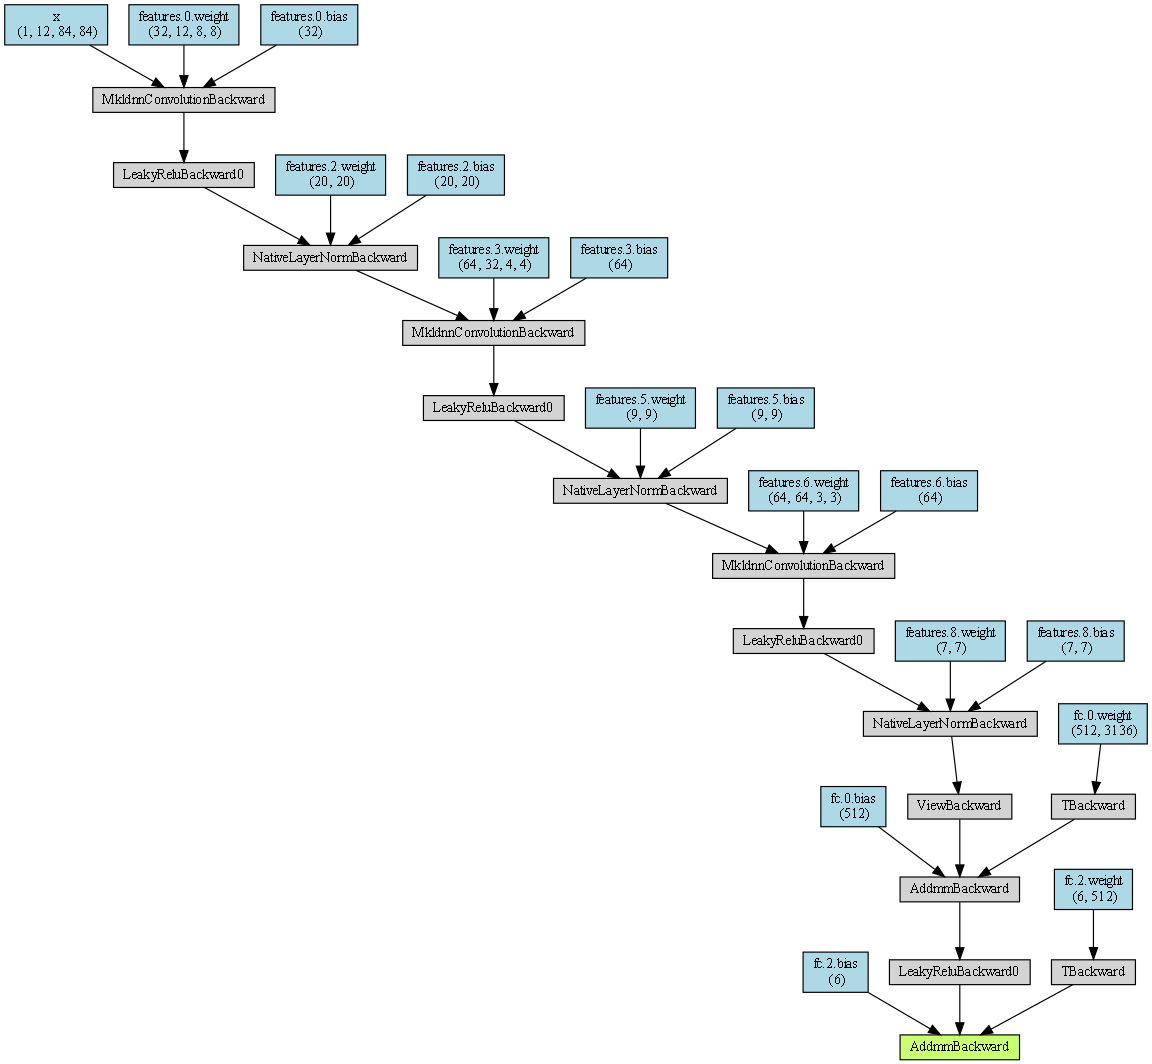
\includegraphics[width=10cm,height=8.8cm]{./resource/model.png}
	\caption{DQN和Double DQN网络参数}
\end{figure}
\begin{figure}[h!]
	\centering
	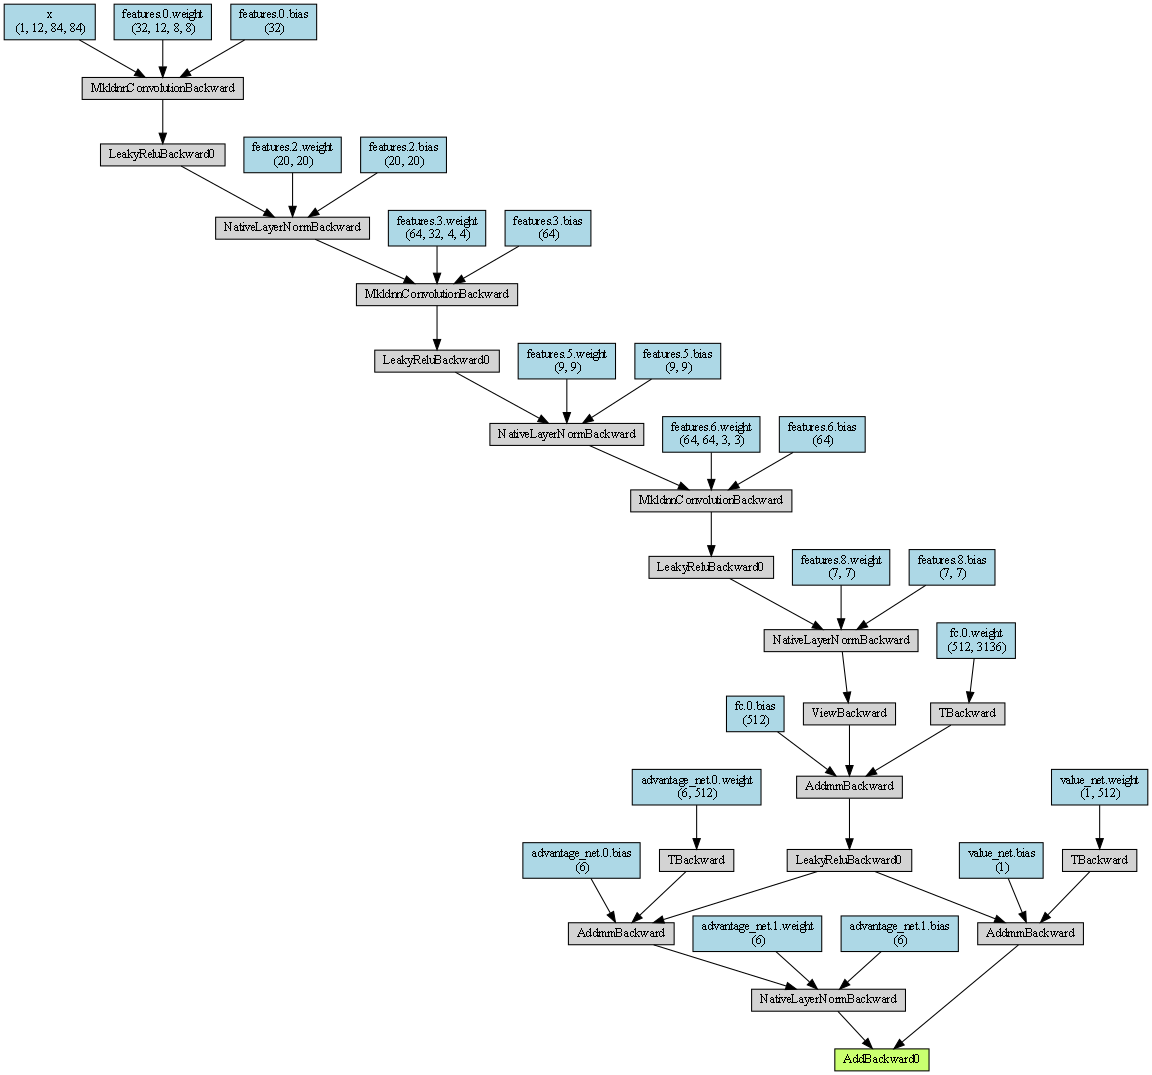
\includegraphics[width=10cm,height=8.8cm]{./resource/dueling_model.png}
	\caption{Dueling DQN网络参数}
\end{figure}
\newpage
\noindent Figure 2和Figure 3分别展示了DQN和Dueling DQN的两种网络参数。在原有卷积神经网络的基础上,我穿插了一些归一化层以提升网络收敛速度,我使用了均方差损失并且改用Adam优化器对网络参数进行优化。
\begin{table}[!h]
	\renewcommand{\arraystretch}{1.1}
	\caption{关键超参数}
	\centering
	\begin{tabular}{ccc}
		\hline
		名称& 默认值& 说明\\
		\hline
		learning\_rate& 1e-5 & 学习率 $\alpha$\\
		gamma& 0.99 & 折扣系数 $\gamma$\\
		frames& 2000000 & 训练总帧数\\
		update\_tar\_interval& 1000 & 目标网络参数更新周期 \\
		batch\_size& 32 & minibatch帧大小\\
		max\_buff& 100000 & 最大帧缓存容量 \\
		win\_reward& 18 & 目标平均奖励 \\
		\hline
	\end{tabular}
\end{table}
\section{实验效果}
\subsection{实验图表展示与分析}
DQN、Double DQN和Dueling DQN的累计奖励和样本训练量之间关系如下。也可以在 \texttt{code} 文件夹下运行 
\texttt{tensorboard --logdir ./model} 并在浏览器中打开链接查看详细的训练过程。\\
\begin{figure}[h!]
	\centering
	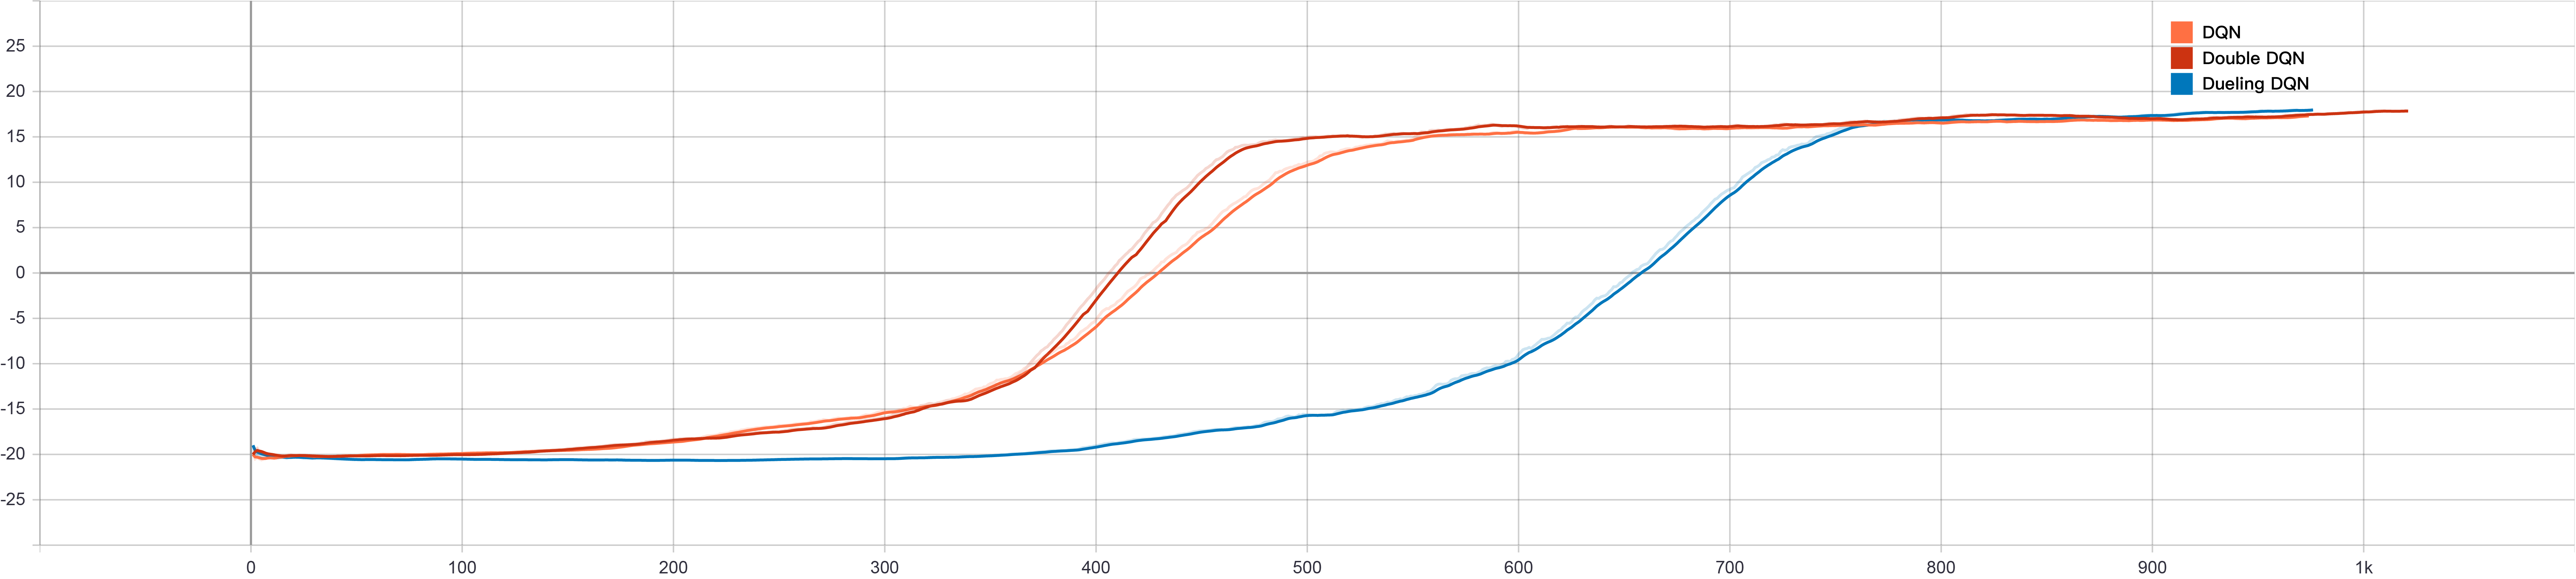
\includegraphics[width=14cm,height=3cm]{./resource/Best 100-episodes average reward.png}
	\caption{最优平均奖励}
\end{figure}
\newpage
\begin{figure}[h!]
	\centering
	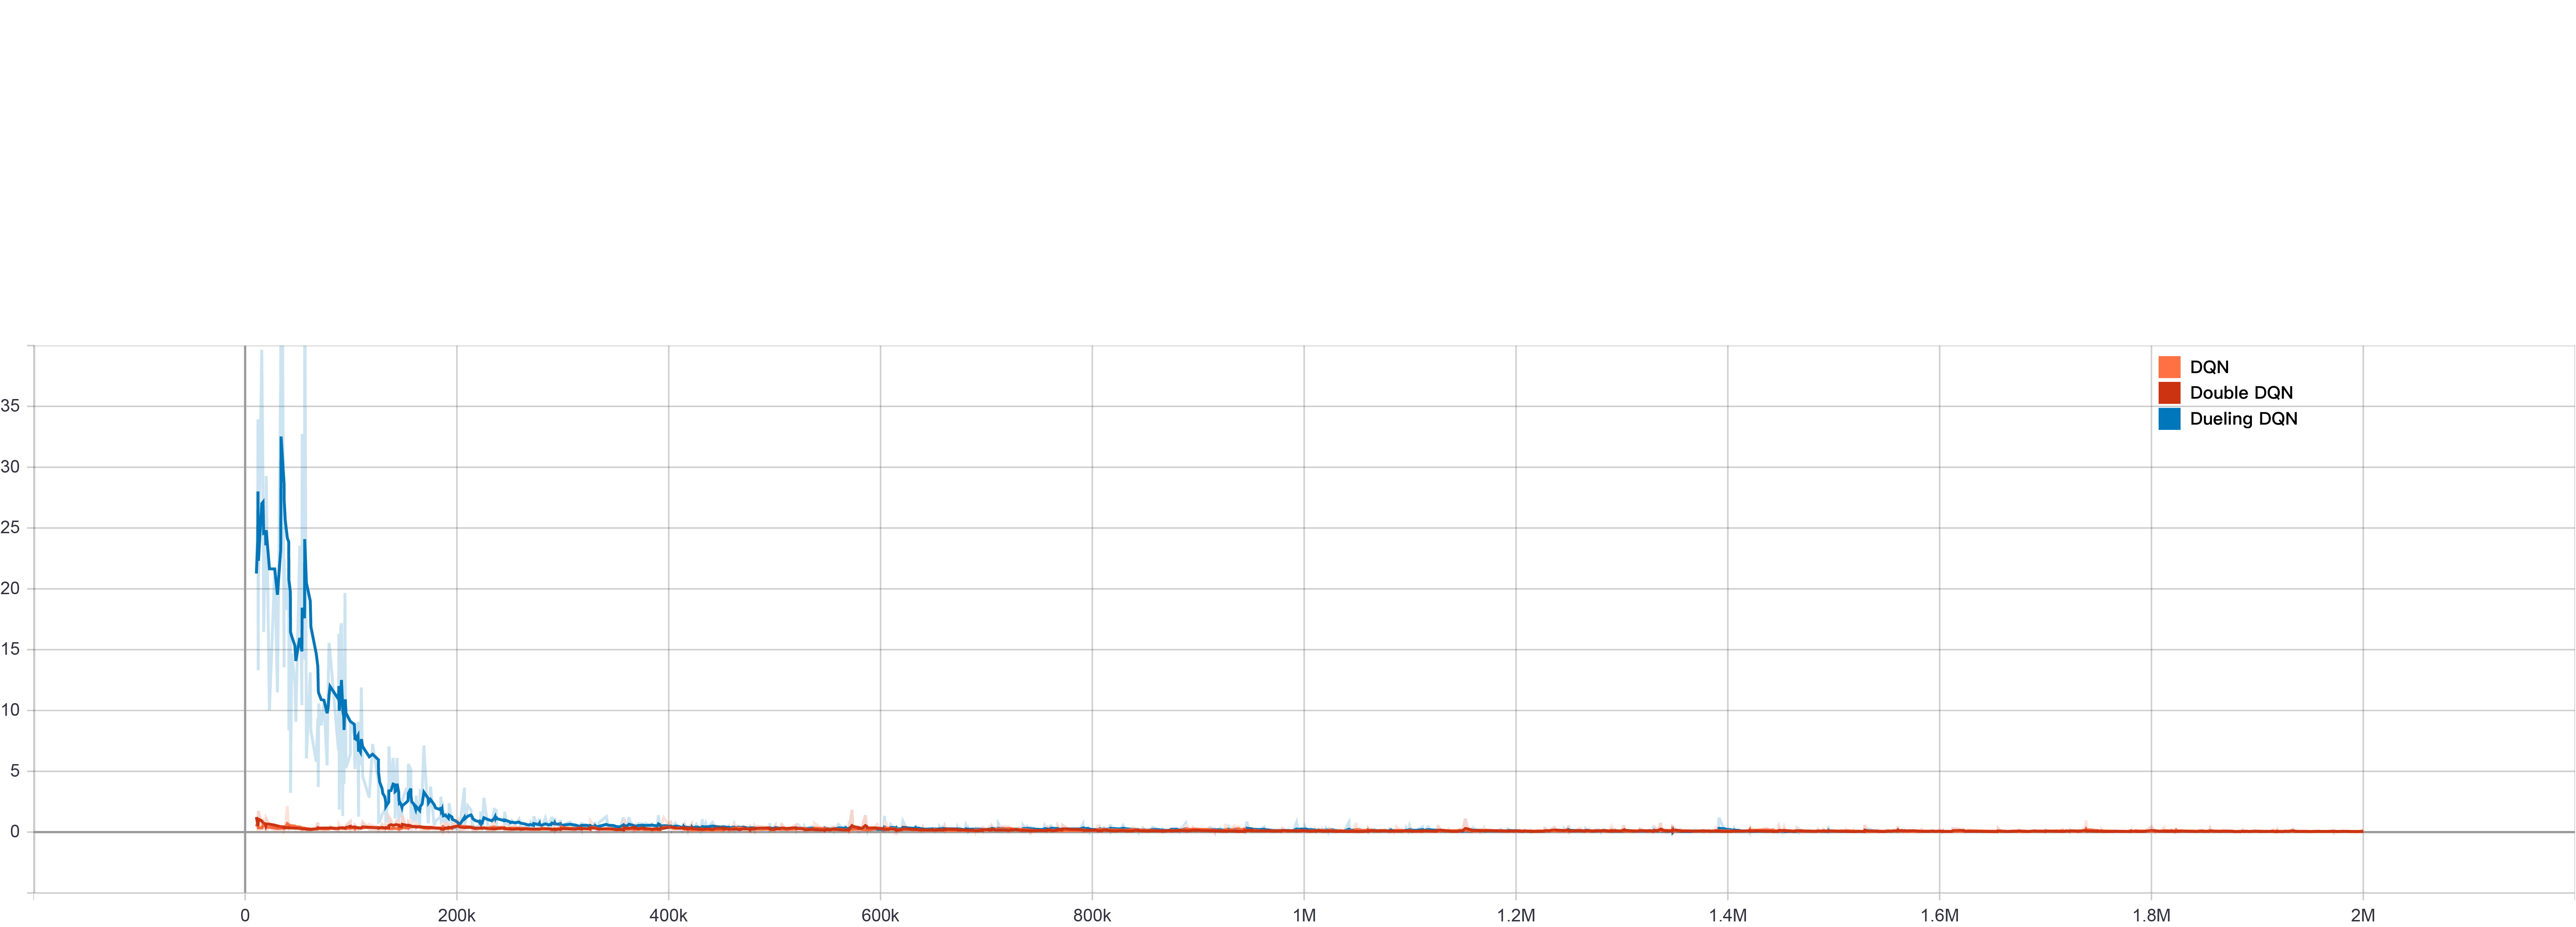
\includegraphics[width=14cm,height=5cm]{./resource/Loss per frame.png}
	\caption{每帧损失}
\end{figure}
\begin{figure}[h!]
	\centering
	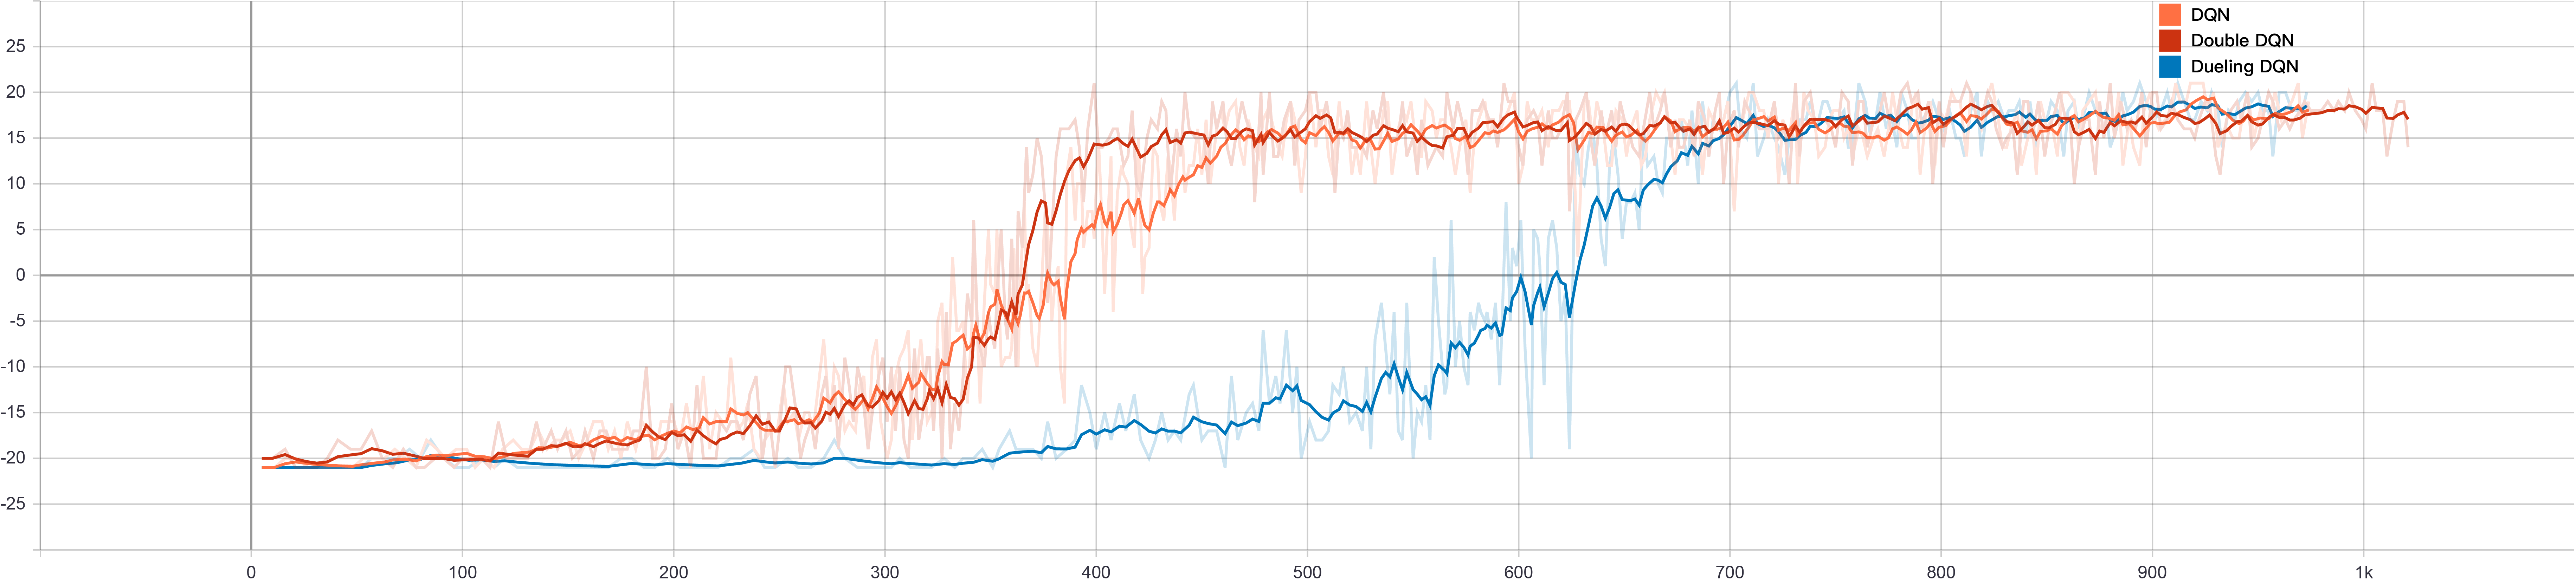
\includegraphics[width=14cm,height=3cm]{./resource/Reward per episode.png}
	\caption{平均奖励}
\end{figure}

\section{小结}
\subsection{关于算法本身}
\subsection{关于实验过程}
\newpage
\renewcommand\refname{参考文献}
\begin{thebibliography}{99}
	\bibitem{ref1}Mnih V, Kavukcuoglu K, Silver D, et al. Playing atari with deep reinforcement learning[J]. arXiv preprint arXiv:1312.5602, 2013.
	\bibitem{ref2}Van Hasselt H, Guez A, Silver D. Deep reinforcement learning with double q-learning[J]. arXiv preprint arXiv:1509.06461, 2015.
	\bibitem{ref3}Wang Z, Schaul T, Hessel M, et al. Dueling network architectures for deep reinforcement learning[C]//International conference on machine learning. PMLR, 2016: 1995-2003.
	\bibitem{ref4}Schaul T, Quan J, Antonoglou I, et al. Prioritized experience replay[J]. arXiv preprint arXiv:1511.05952, 2015.
	\bibitem{ref5}Watkins C J C H, Dayan P. Q-learning[J]. Machine learning, 1992, 8(3-4): 279-292.
\end{thebibliography}
\end{CJK}
\end{document}
